\section{Referencia de la Estructura sentencia}
\label{structsentencia}\index{sentencia@{sentencia}}
Clase de almacenamiento de raiz de un arbol de sentencias en el AST, siendo a su vez una lista.  


{\tt \#include $<$ast.h$>$}

Diagrama de colaboraci\'{o}n para sentencia:\begin{figure}[H]
\begin{center}
\leavevmode
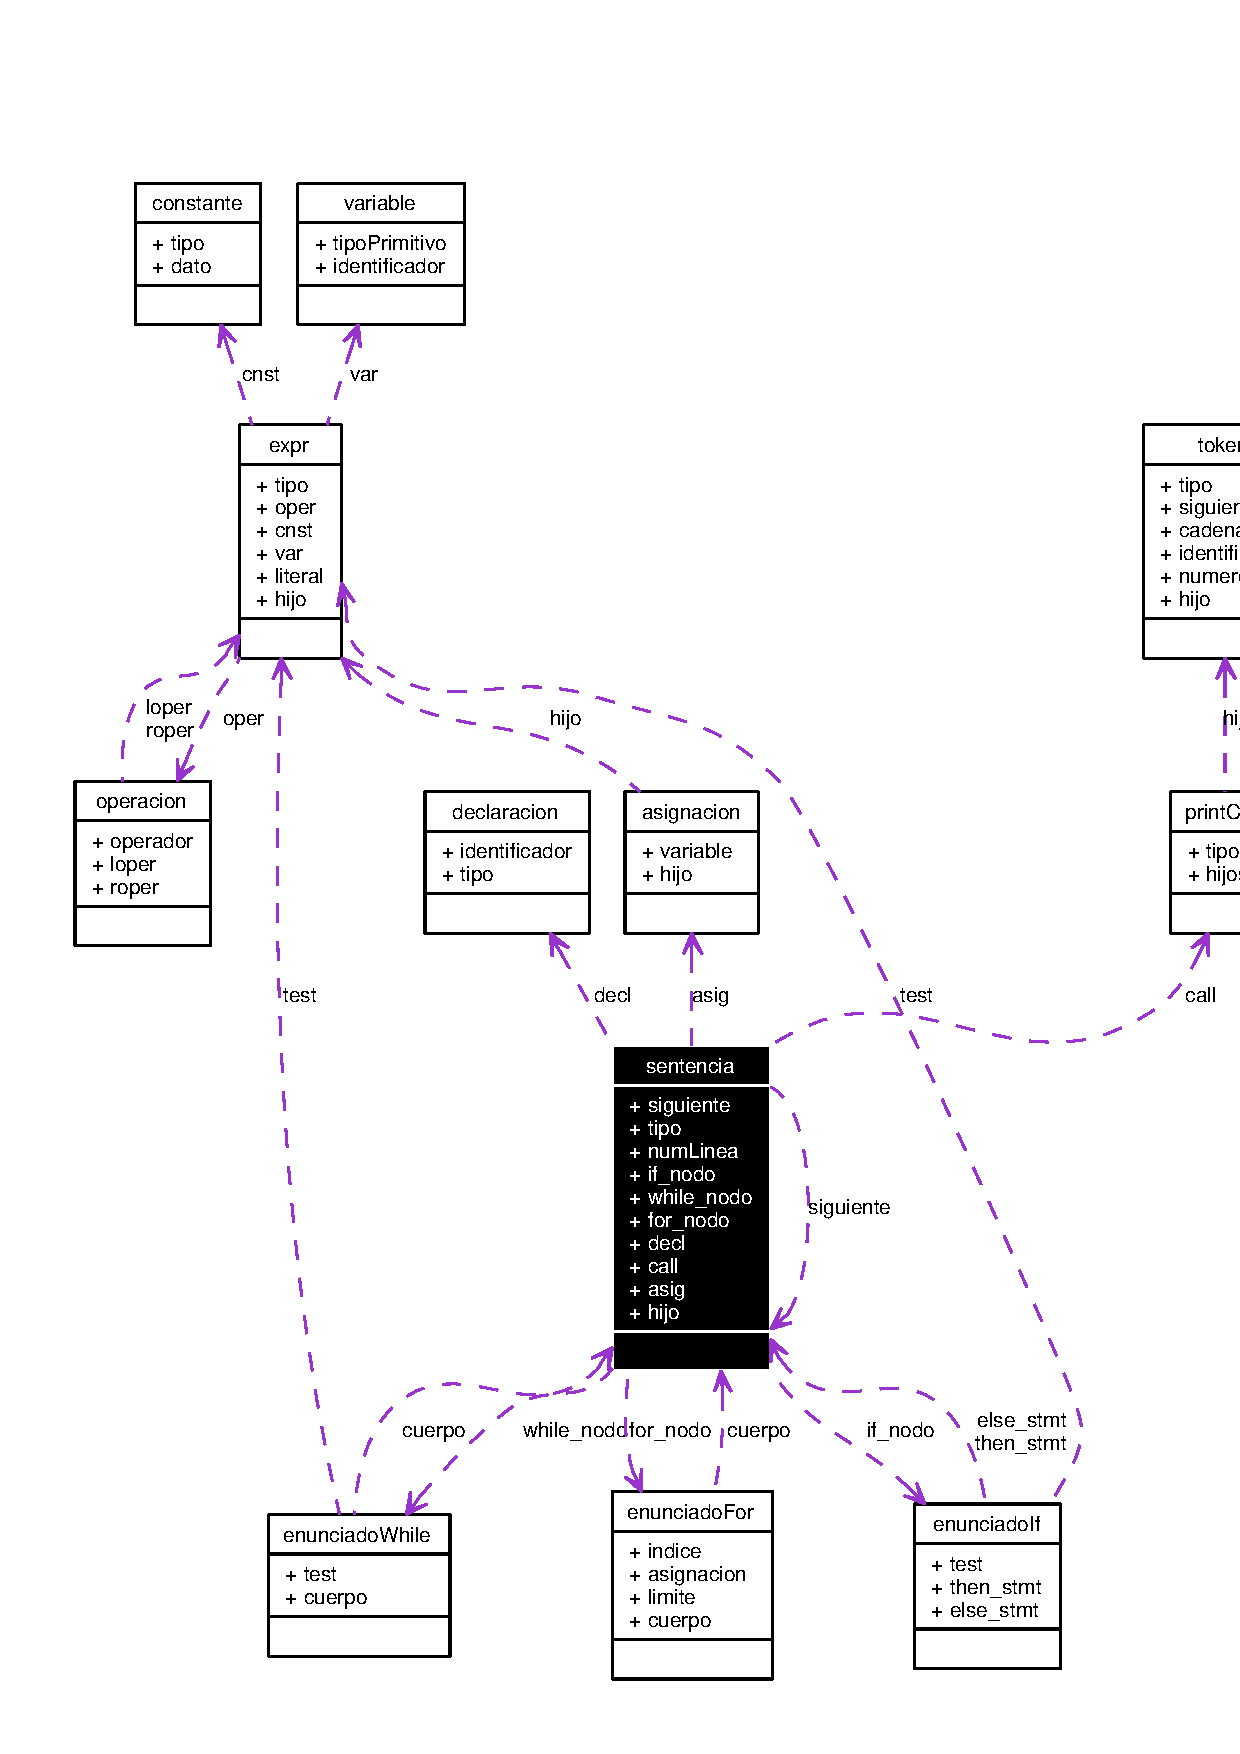
\includegraphics[width=343pt]{structsentencia__coll__graph}
\end{center}
\end{figure}
\subsection*{Atributos p\'{u}blicos}
\begin{CompactItemize}
\item 
{\bf sentencia} $\ast$ {\bf siguiente}
\begin{CompactList}\small\item\em Sentencia siguiente a evaluar. \item\end{CompactList}\item 
int {\bf tipo}
\begin{CompactList}\small\item\em Tipo de sentencia. \item\end{CompactList}\item 
int {\bf num\-Linea}
\begin{CompactList}\small\item\em Numero de linea en donde se encontraba la sentecia, esto es para escribir a archivo de error. \item\end{CompactList}\item 
\begin{tabbing}
xx\=xx\=xx\=xx\=xx\=xx\=xx\=xx\=xx\=\kill
union \{\\
\>{\bf enunciadoIf} $\ast$ {\bf if\_nodo}\\
\>{\bf enunciadoWhile} $\ast$ {\bf while\_nodo}\\
\>{\bf enunciadoFor} $\ast$ {\bf for\_nodo}\\
\>{\bf declaracion} $\ast$ {\bf decl}\\
\>{\bf printCall} $\ast$ {\bf call}\\
\>{\bf asignacion} $\ast$ {\bf asig}\\
\} {\bf hijo}\\

\end{tabbing}\begin{CompactList}\small\item\em Nodos hijos del arbol de sentencias. \item\end{CompactList}\end{CompactItemize}


\subsection{Descripci\'{o}n detallada}
Clase de almacenamiento de raiz de un arbol de sentencias en el AST, siendo a su vez una lista. 



Definici\'{o}n en la l\'{\i}nea 227 del archivo ast.h.

\subsection{Documentaci\'{o}n de los datos miembro}
\index{sentencia@{sentencia}!asig@{asig}}
\index{asig@{asig}!sentencia@{sentencia}}
\subsubsection{\setlength{\rightskip}{0pt plus 5cm}{\bf asignacion}$\ast$ {\bf sentencia::asig}}\label{structsentencia_o8}




Definici\'{o}n en la l\'{\i}nea 238 del archivo ast.h.\index{sentencia@{sentencia}!call@{call}}
\index{call@{call}!sentencia@{sentencia}}
\subsubsection{\setlength{\rightskip}{0pt plus 5cm}{\bf print\-Call}$\ast$ {\bf sentencia::call}}\label{structsentencia_o7}




Definici\'{o}n en la l\'{\i}nea 237 del archivo ast.h.\index{sentencia@{sentencia}!decl@{decl}}
\index{decl@{decl}!sentencia@{sentencia}}
\subsubsection{\setlength{\rightskip}{0pt plus 5cm}{\bf declaracion}$\ast$ {\bf sentencia::decl}}\label{structsentencia_o6}




Definici\'{o}n en la l\'{\i}nea 236 del archivo ast.h.\index{sentencia@{sentencia}!for_nodo@{for\_\-nodo}}
\index{for_nodo@{for\_\-nodo}!sentencia@{sentencia}}
\subsubsection{\setlength{\rightskip}{0pt plus 5cm}{\bf enunciado\-For}$\ast$ {\bf sentencia::for\_\-nodo}}\label{structsentencia_o5}




Definici\'{o}n en la l\'{\i}nea 235 del archivo ast.h.\index{sentencia@{sentencia}!hijo@{hijo}}
\index{hijo@{hijo}!sentencia@{sentencia}}
\subsubsection{\setlength{\rightskip}{0pt plus 5cm}union \{ ... \}  {\bf sentencia::hijo}}\label{structsentencia_o9}


Nodos hijos del arbol de sentencias. 



Referenciado por borrar\-Sentencias(), evaluar\-Sentencia(), y insertar\-Sentencia().\index{sentencia@{sentencia}!if_nodo@{if\_\-nodo}}
\index{if_nodo@{if\_\-nodo}!sentencia@{sentencia}}
\subsubsection{\setlength{\rightskip}{0pt plus 5cm}{\bf enunciado\-If}$\ast$ {\bf sentencia::if\_\-nodo}}\label{structsentencia_o3}




Definici\'{o}n en la l\'{\i}nea 233 del archivo ast.h.\index{sentencia@{sentencia}!numLinea@{numLinea}}
\index{numLinea@{numLinea}!sentencia@{sentencia}}
\subsubsection{\setlength{\rightskip}{0pt plus 5cm}int {\bf sentencia::num\-Linea}}\label{structsentencia_o2}


Numero de linea en donde se encontraba la sentecia, esto es para escribir a archivo de error. 



Definici\'{o}n en la l\'{\i}nea 230 del archivo ast.h.

Referenciado por error(), y insertar\-Sentencia().\index{sentencia@{sentencia}!siguiente@{siguiente}}
\index{siguiente@{siguiente}!sentencia@{sentencia}}
\subsubsection{\setlength{\rightskip}{0pt plus 5cm}{\bf sentencia}$\ast$ {\bf sentencia::siguiente}}\label{structsentencia_o0}


Sentencia siguiente a evaluar. 



Definici\'{o}n en la l\'{\i}nea 228 del archivo ast.h.

Referenciado por borrar\-Sentencias(), concatenar\-Sentencia(), insertar\-Sentencia(), y recorrer\-Sentencia().\index{sentencia@{sentencia}!tipo@{tipo}}
\index{tipo@{tipo}!sentencia@{sentencia}}
\subsubsection{\setlength{\rightskip}{0pt plus 5cm}int {\bf sentencia::tipo}}\label{structsentencia_o1}


Tipo de sentencia. 



Definici\'{o}n en la l\'{\i}nea 229 del archivo ast.h.

Referenciado por borrar\-Sentencias(), evaluar\-Sentencia(), y insertar\-Sentencia().\index{sentencia@{sentencia}!while_nodo@{while\_\-nodo}}
\index{while_nodo@{while\_\-nodo}!sentencia@{sentencia}}
\subsubsection{\setlength{\rightskip}{0pt plus 5cm}{\bf enunciado\-While}$\ast$ {\bf sentencia::while\_\-nodo}}\label{structsentencia_o4}




Definici\'{o}n en la l\'{\i}nea 234 del archivo ast.h.

La documentaci\'{o}n para esta estructura fu\'{e} generada a partir del siguiente archivo:\begin{CompactItemize}
\item 
/media/docs/progra/c++/compiladores1/proy2/godzilla/src/{\bf ast.h}\end{CompactItemize}
